\chapter{Mechanical Parts}
\graphicspath{{./Mechanical/img/}}



\section{Signs}

For the signs, which have to be recognized by the software, sign posts (see in figure \vref{figure:signs}) were created.
They consist of a round plate with a thread on the side, a round stand with a thread in the middle and a staff connecting
with a thread on each side to connect them.

The diameter of the sign is 15 cm and it's overall height measures 50 cm.

The signs graphic, a standardized european speed limit sign, was taken from 
Wikipedia\footnote{\url{http://upload.wikimedia.org/wikipedia/commons/archive/2/2e/20120617230605!Zeichen_274-56.svg}}
and modified to have an arrow in it's center. 

 \begin{figure}[htp]
\begin{center}
  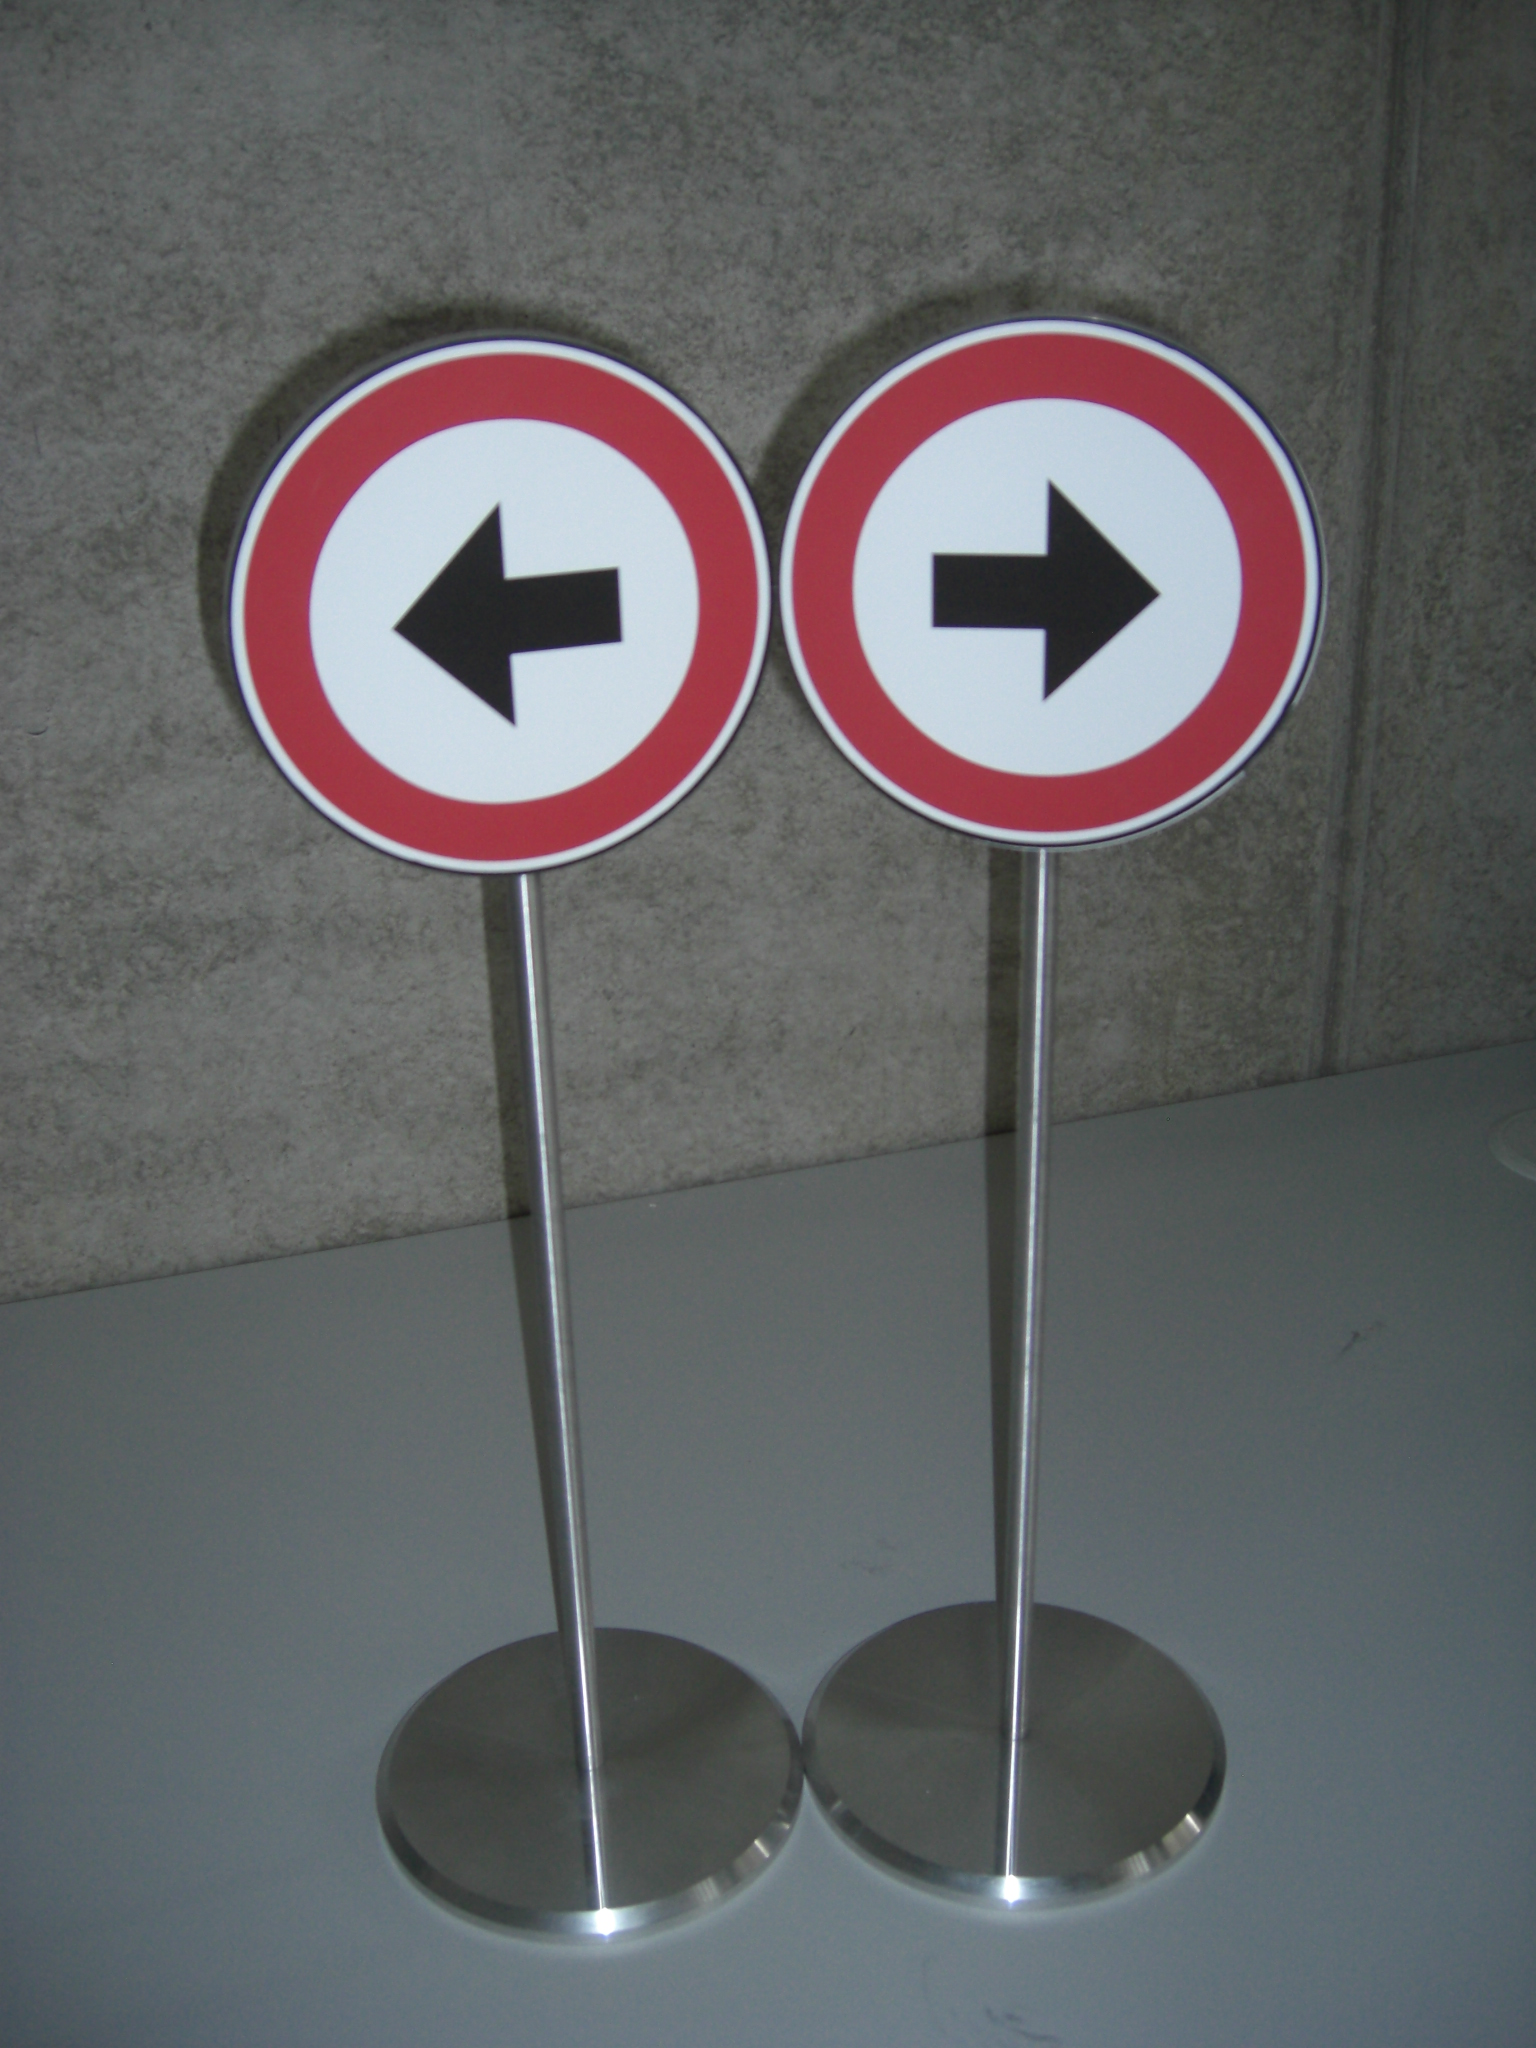
\includegraphics[width=\textwidth/3]{signs.jpg}
  \caption{Signs for Recognition}
  \label{figure:signs}
\end{center}
\end{figure}

\section{Robot Update}

For using the Kinect with the given Pioneer 3dx it was necessary to fix the camera at the robot.
Due to some lacks of the previous laptop stand, it was decided to completely rework it.

The old laptop stand had problems with rust and weight,
because it is made of steel. Another disadvantage is, that the Laptop bracket, which keeps the 
controlling laptop from tilting, is made out of aluminium and has sharp corners. This can lead
to a damage of the laptops case, especially when the laptop is removed from the stand. 

The new stand as seen in figure \vref{figure:laptop_stand} and \vref{figure:laptop_stand_side} is now lower in
weight and doesn't rust because the main tray is made out of aluminium. The new laptop brackets 
(see in figure \vref{figure:laptop_bracket}) are made out acrylic plastic and have rounded down edges and corners, 
so it's mostly impossible to damage the laptops casing. The stand also features a Kinect holder 
(see in figure \vref{figure:kc_hold}) from where the Kinect can be easily dismounted. For dismounting, 
it is only necessary to loosen two wing nuts. A possible disadvantage of the new design, a bad visibility of
the status LEDs of the laser scanner, could be foreseen within the design process. 
To avoid this design flaw, a viewing window was constructed into the tray (see in figure \vref{figure:viewingwindow}). 
If using a 15" laptop for controlling the robot, the viewing window is completely uncovered 
(see in figure \vref{figure:viewingwindowlaptop}). Normally a newer netbook can be considered to be 
adequate in performance to control the robot. Another feature is the invented cable box 
(shown in figure \vref{figure:laptop_stand_side}), which holds the very long cable of the Kinect camera. 
Additionally the form of the main tray fits the form of the robots tray, making it look in a more professional 
way and like done by the manufacturer. The only thing to improve this would be, to paint the tray in the 
same dark grey color, which is used for the robots tray.

\begin{figure}[htp]
\begin{center}
  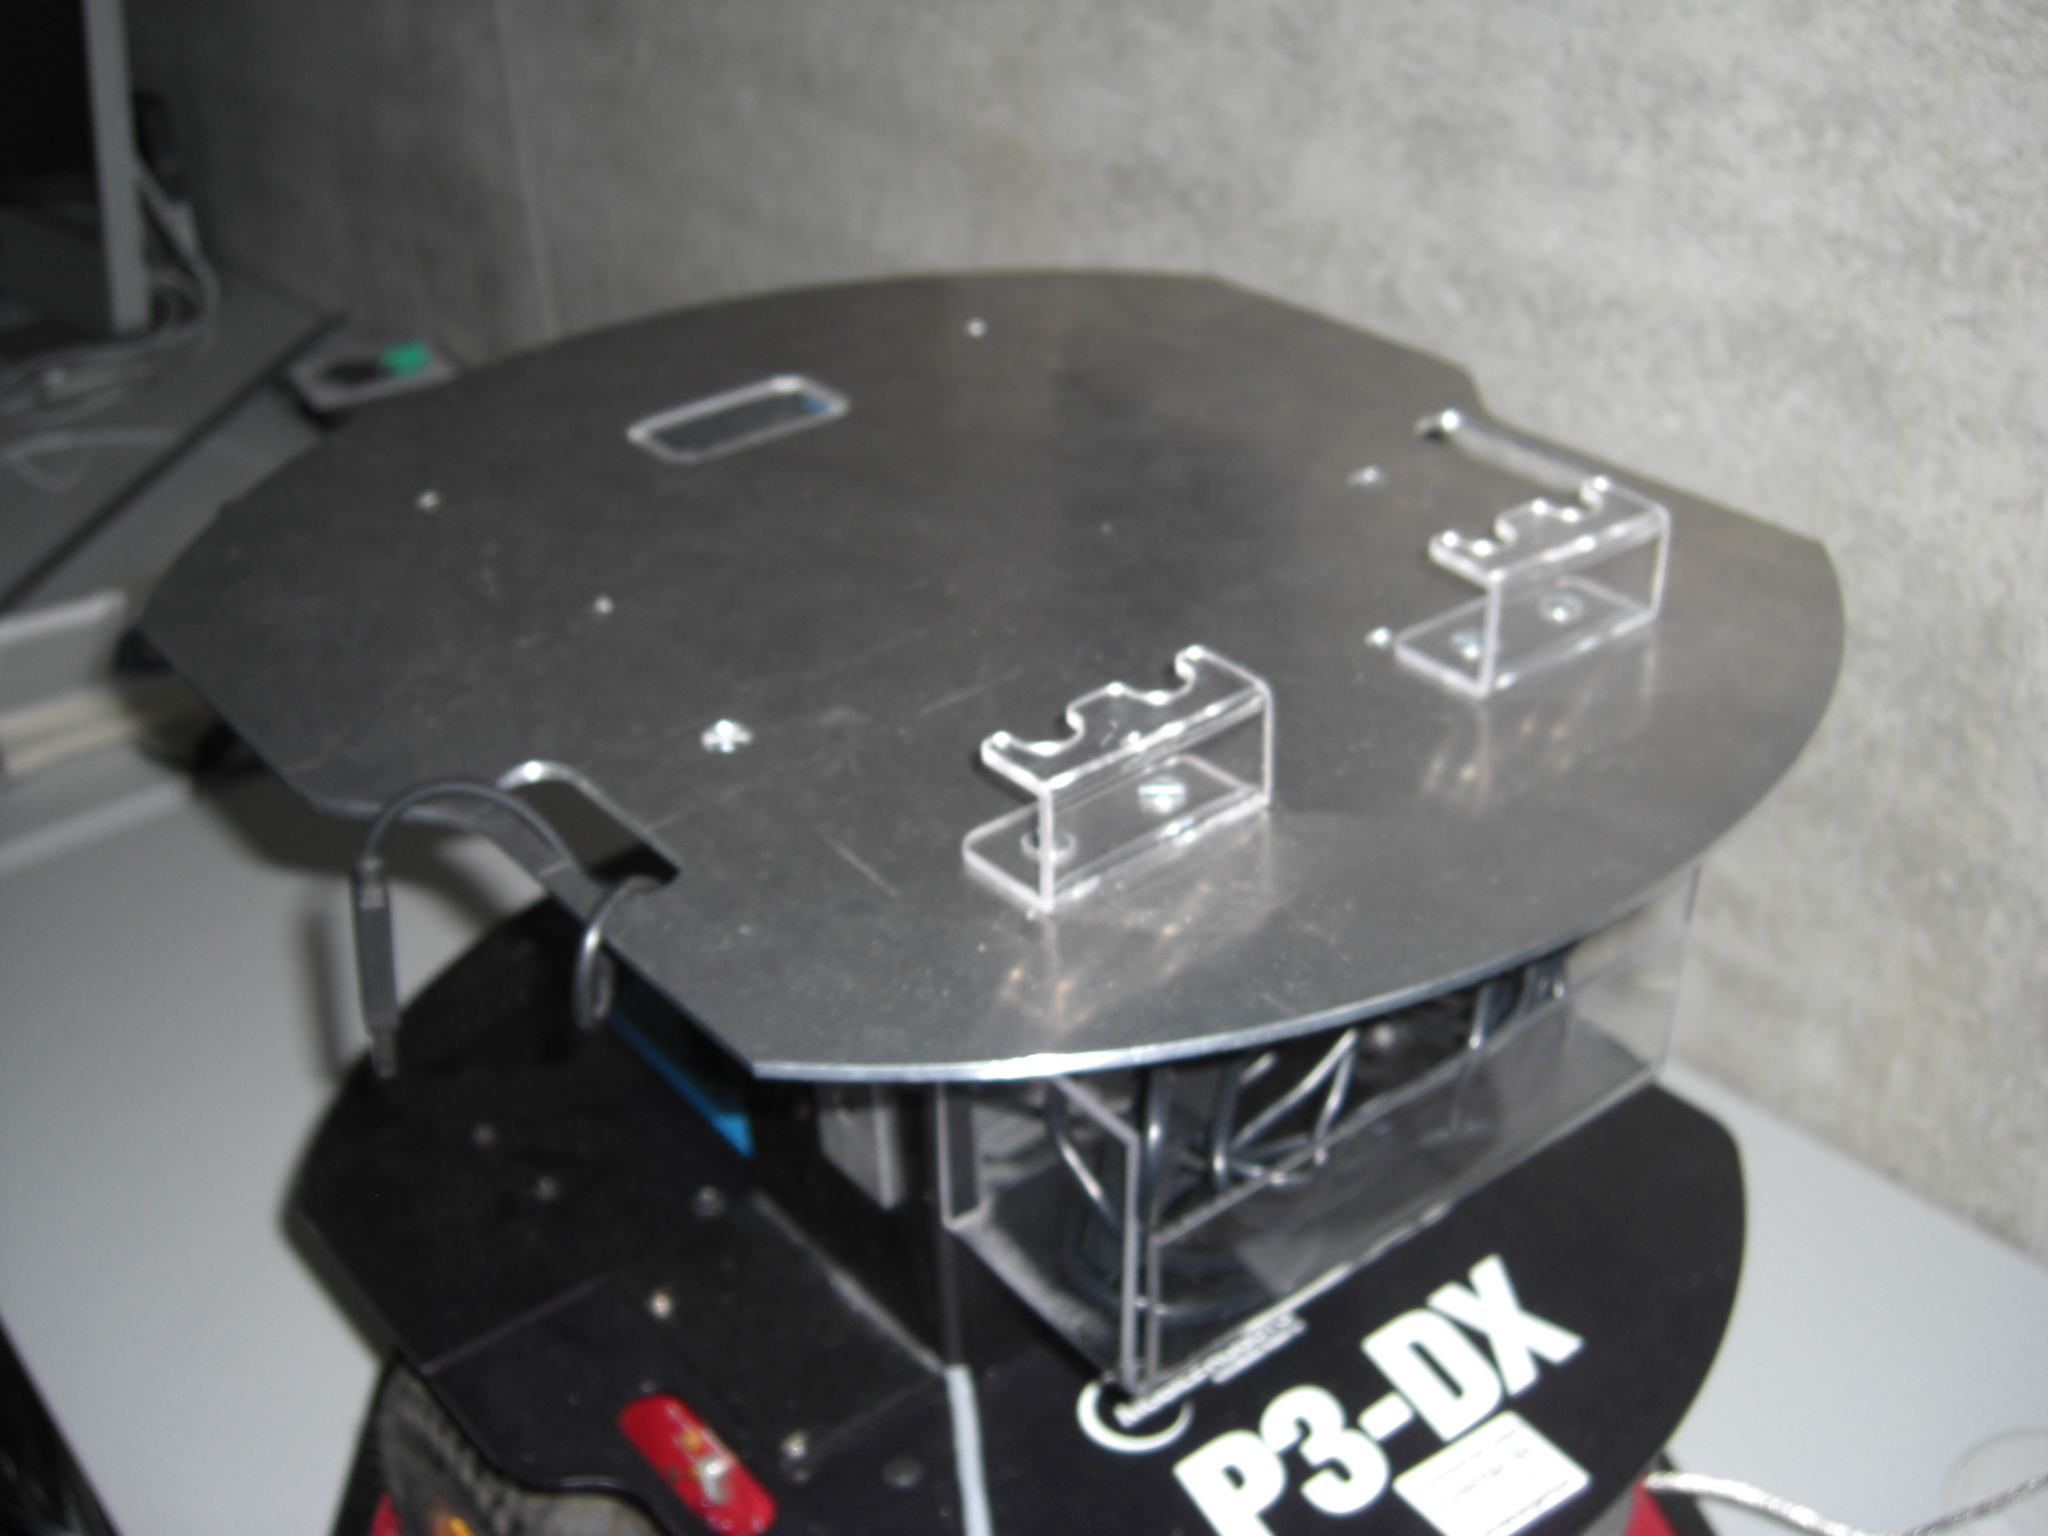
\includegraphics[width=\textwidth/2]{laptop_stand.jpg}
  \caption{Laptop Stand}
  \label{figure:laptop_stand}
\end{center}
\end{figure}
\begin{figure}[htp]
\begin{center}
  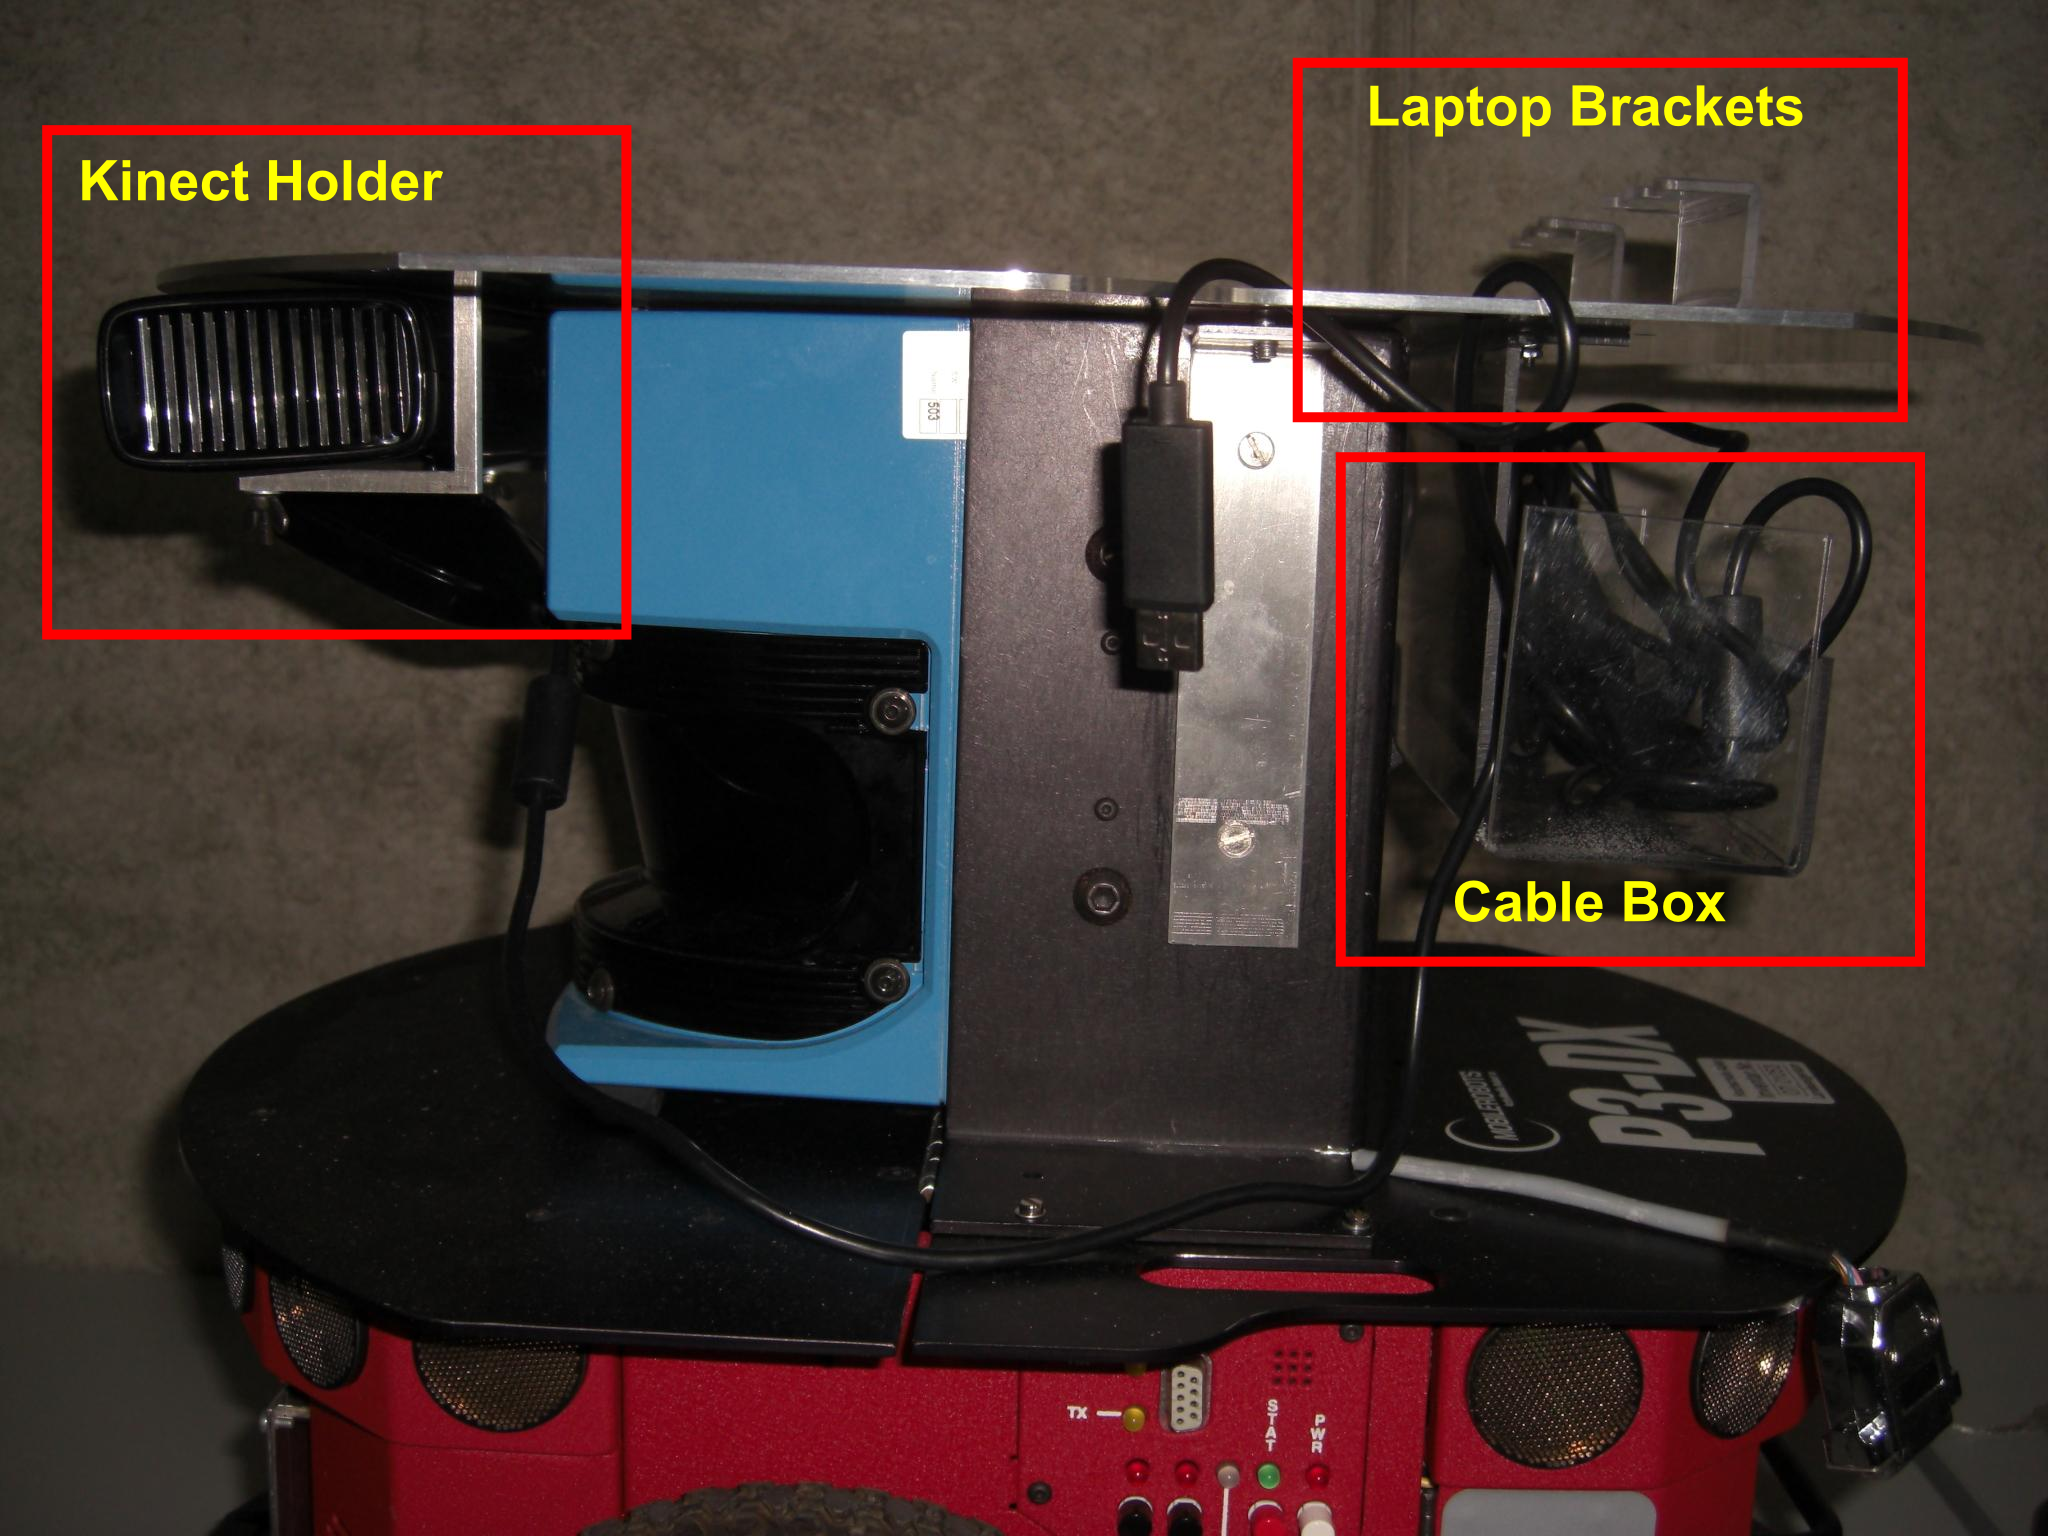
\includegraphics[width=\textwidth]{laptop_stand_side.png}
  \caption{Laptop Stand Feature Overview}
  \label{figure:laptop_stand_side}
\end{center}
\end{figure}


\begin{figure}[htp]
\begin{center}
  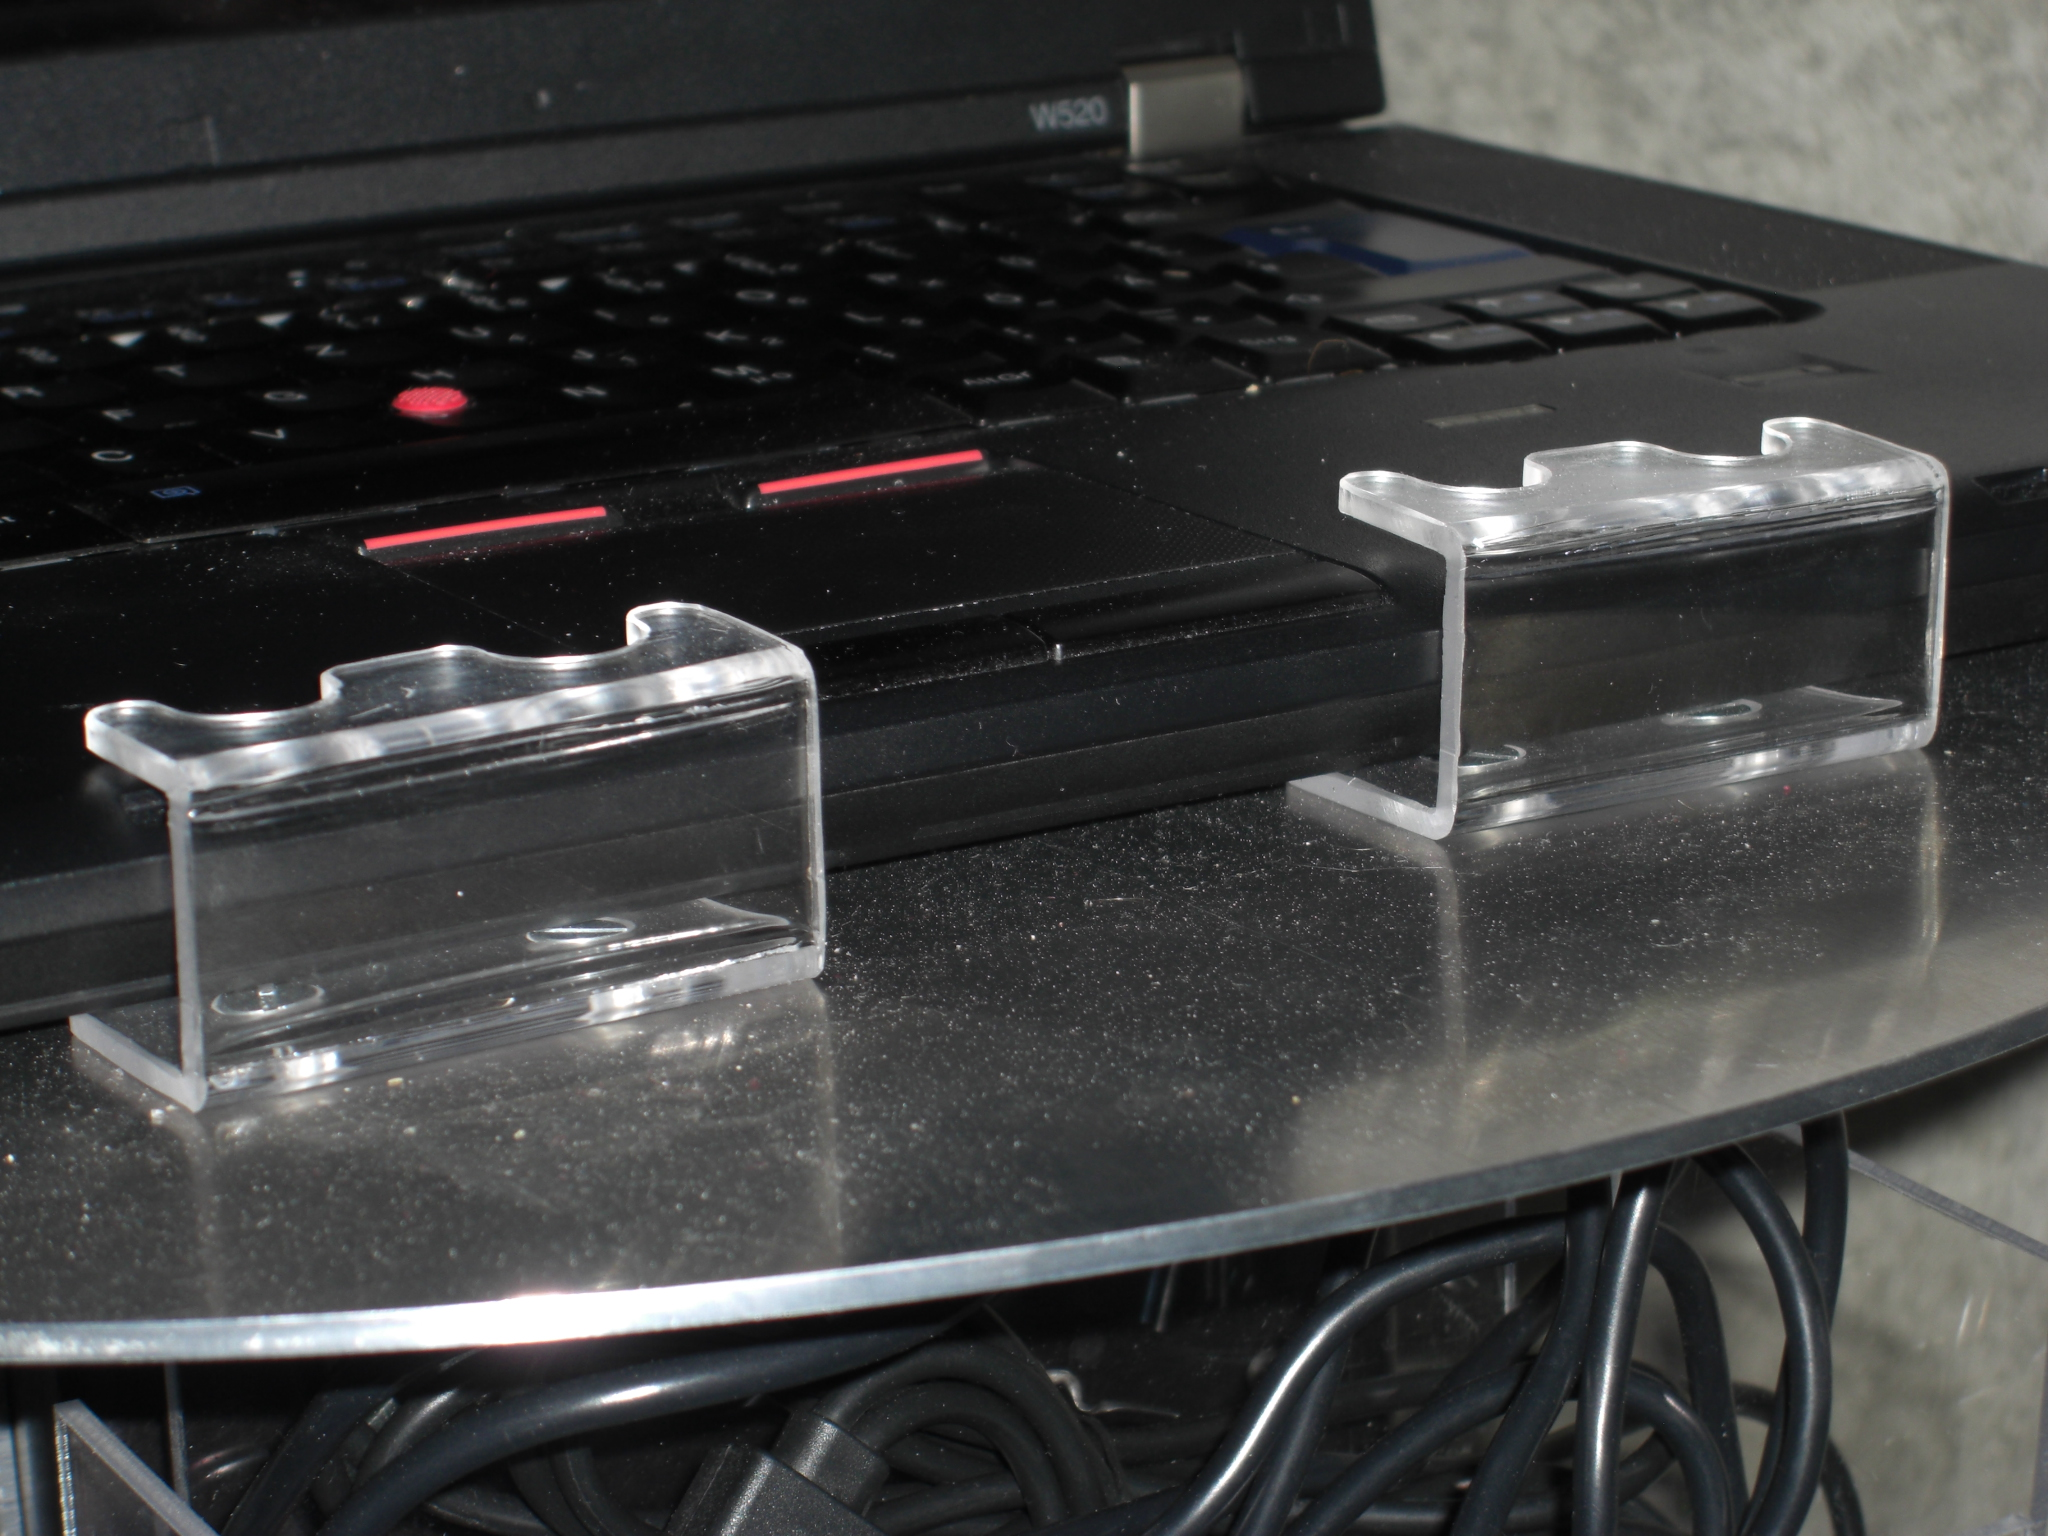
\includegraphics[width=\textwidth/2]{laptop_bracket.jpg}
  \caption{Holding Brackets for Laptops}
  \label{figure:laptop_bracket}
\end{center}
\end{figure}
\begin{figure}[htp]
\begin{center}
  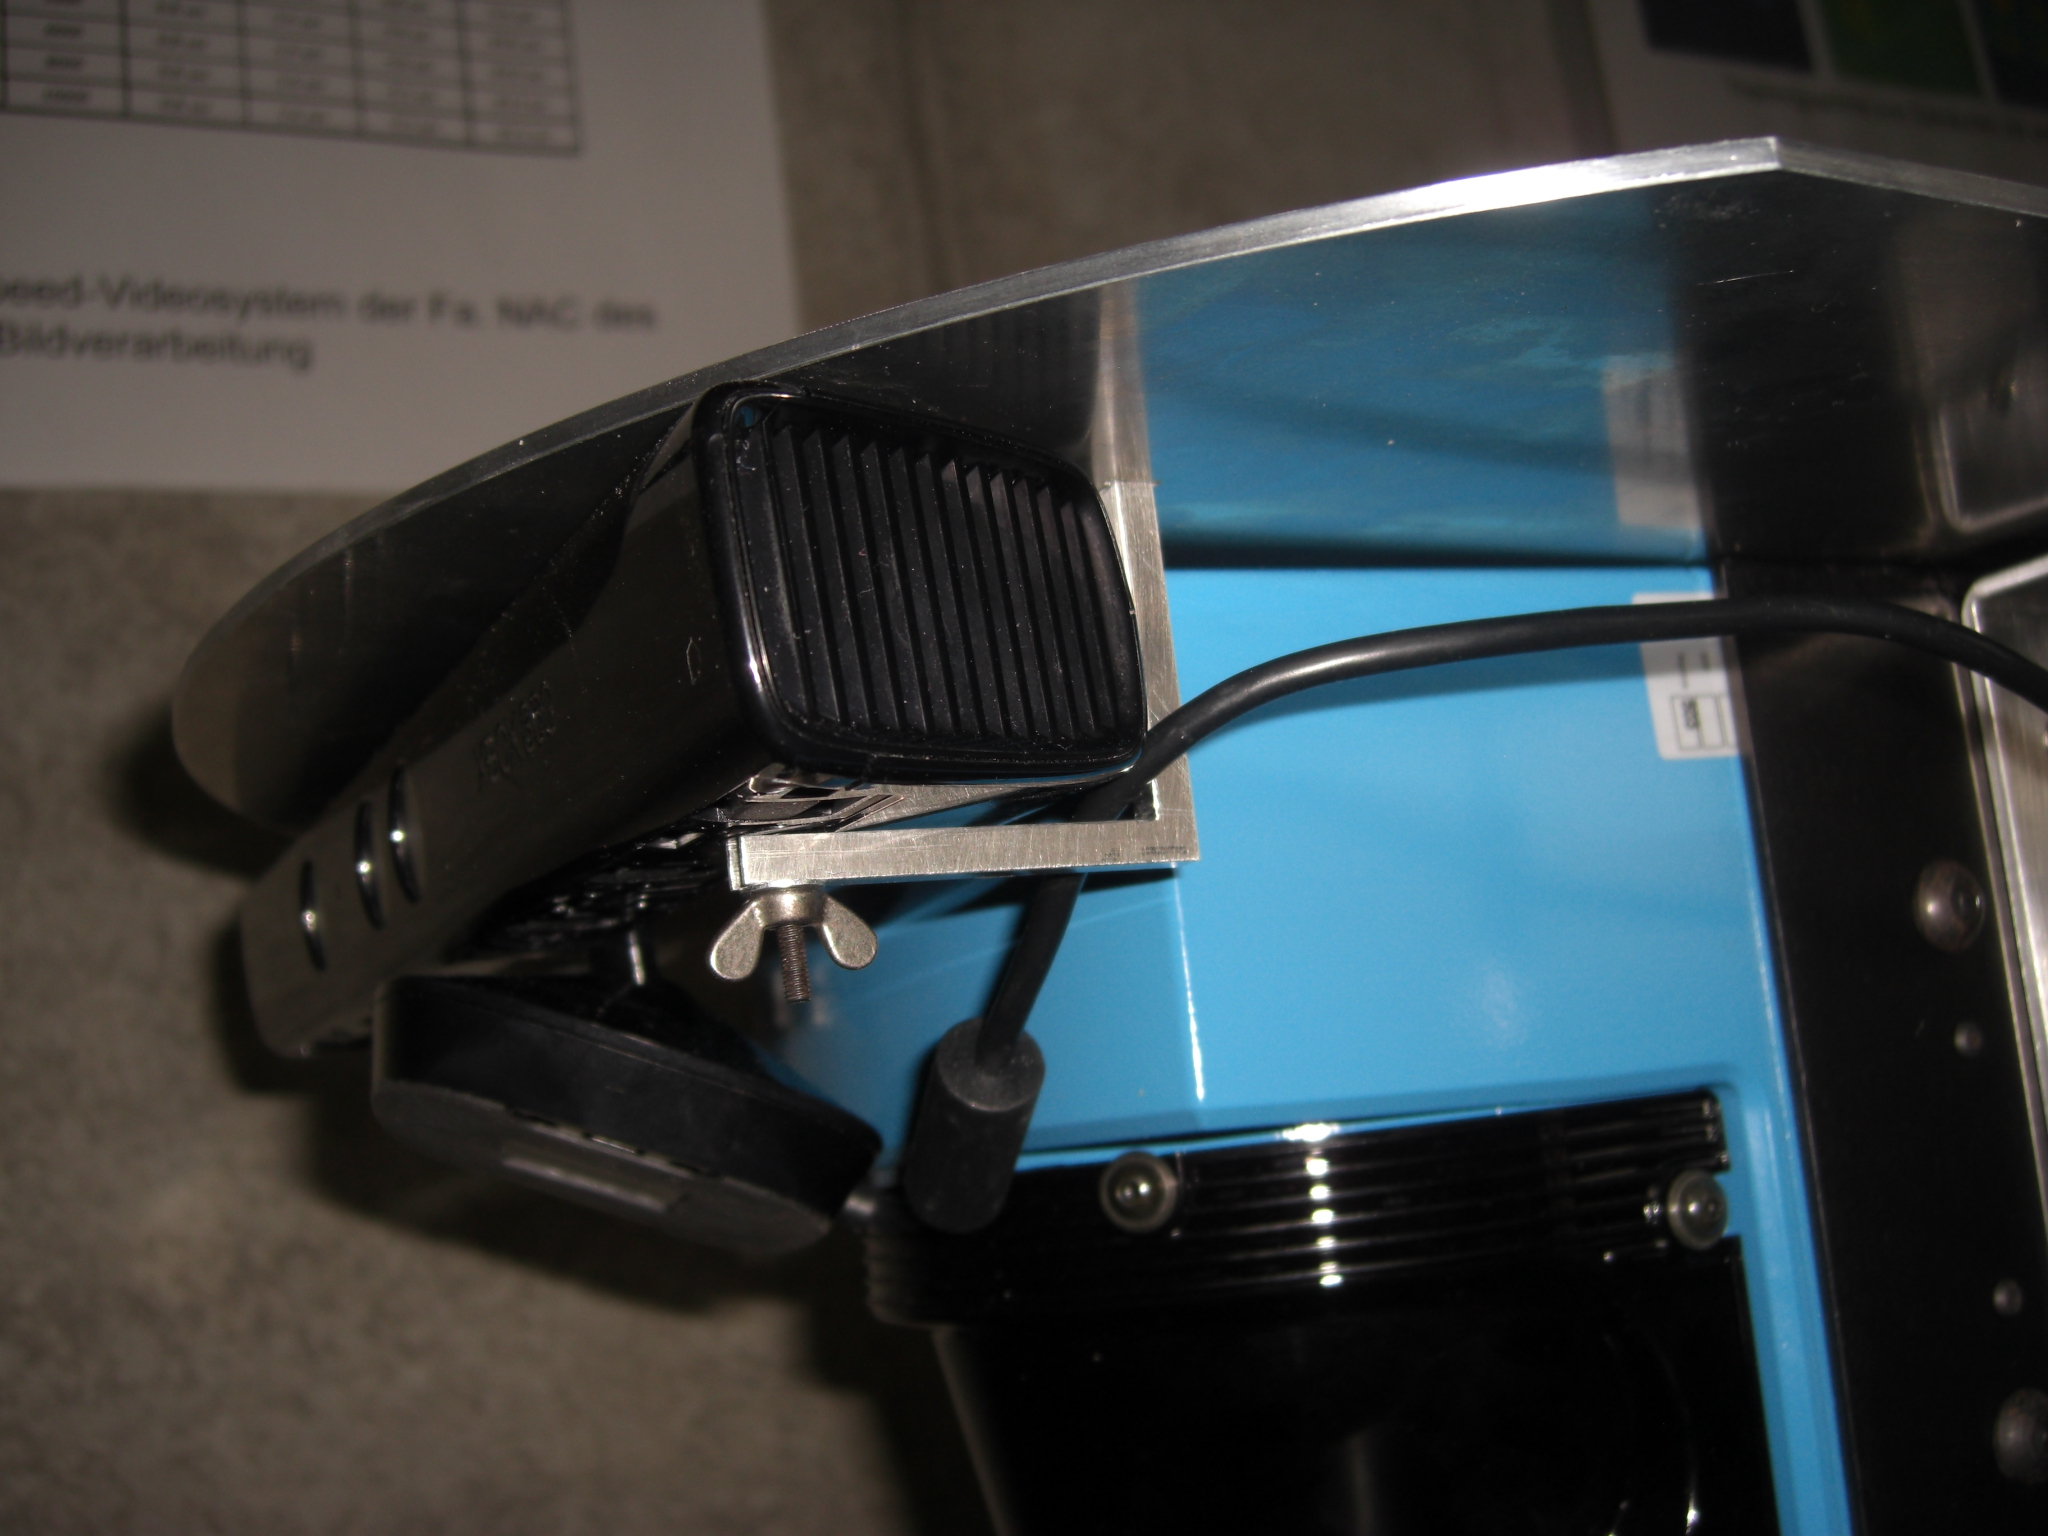
\includegraphics[width=\textwidth]{kinect_bracket.jpg}
  \caption{Kinect Camera Holder}
  \label{figure:kc_hold}
\end{center}
\end{figure}

\begin{figure}[htp]
\begin{center}
  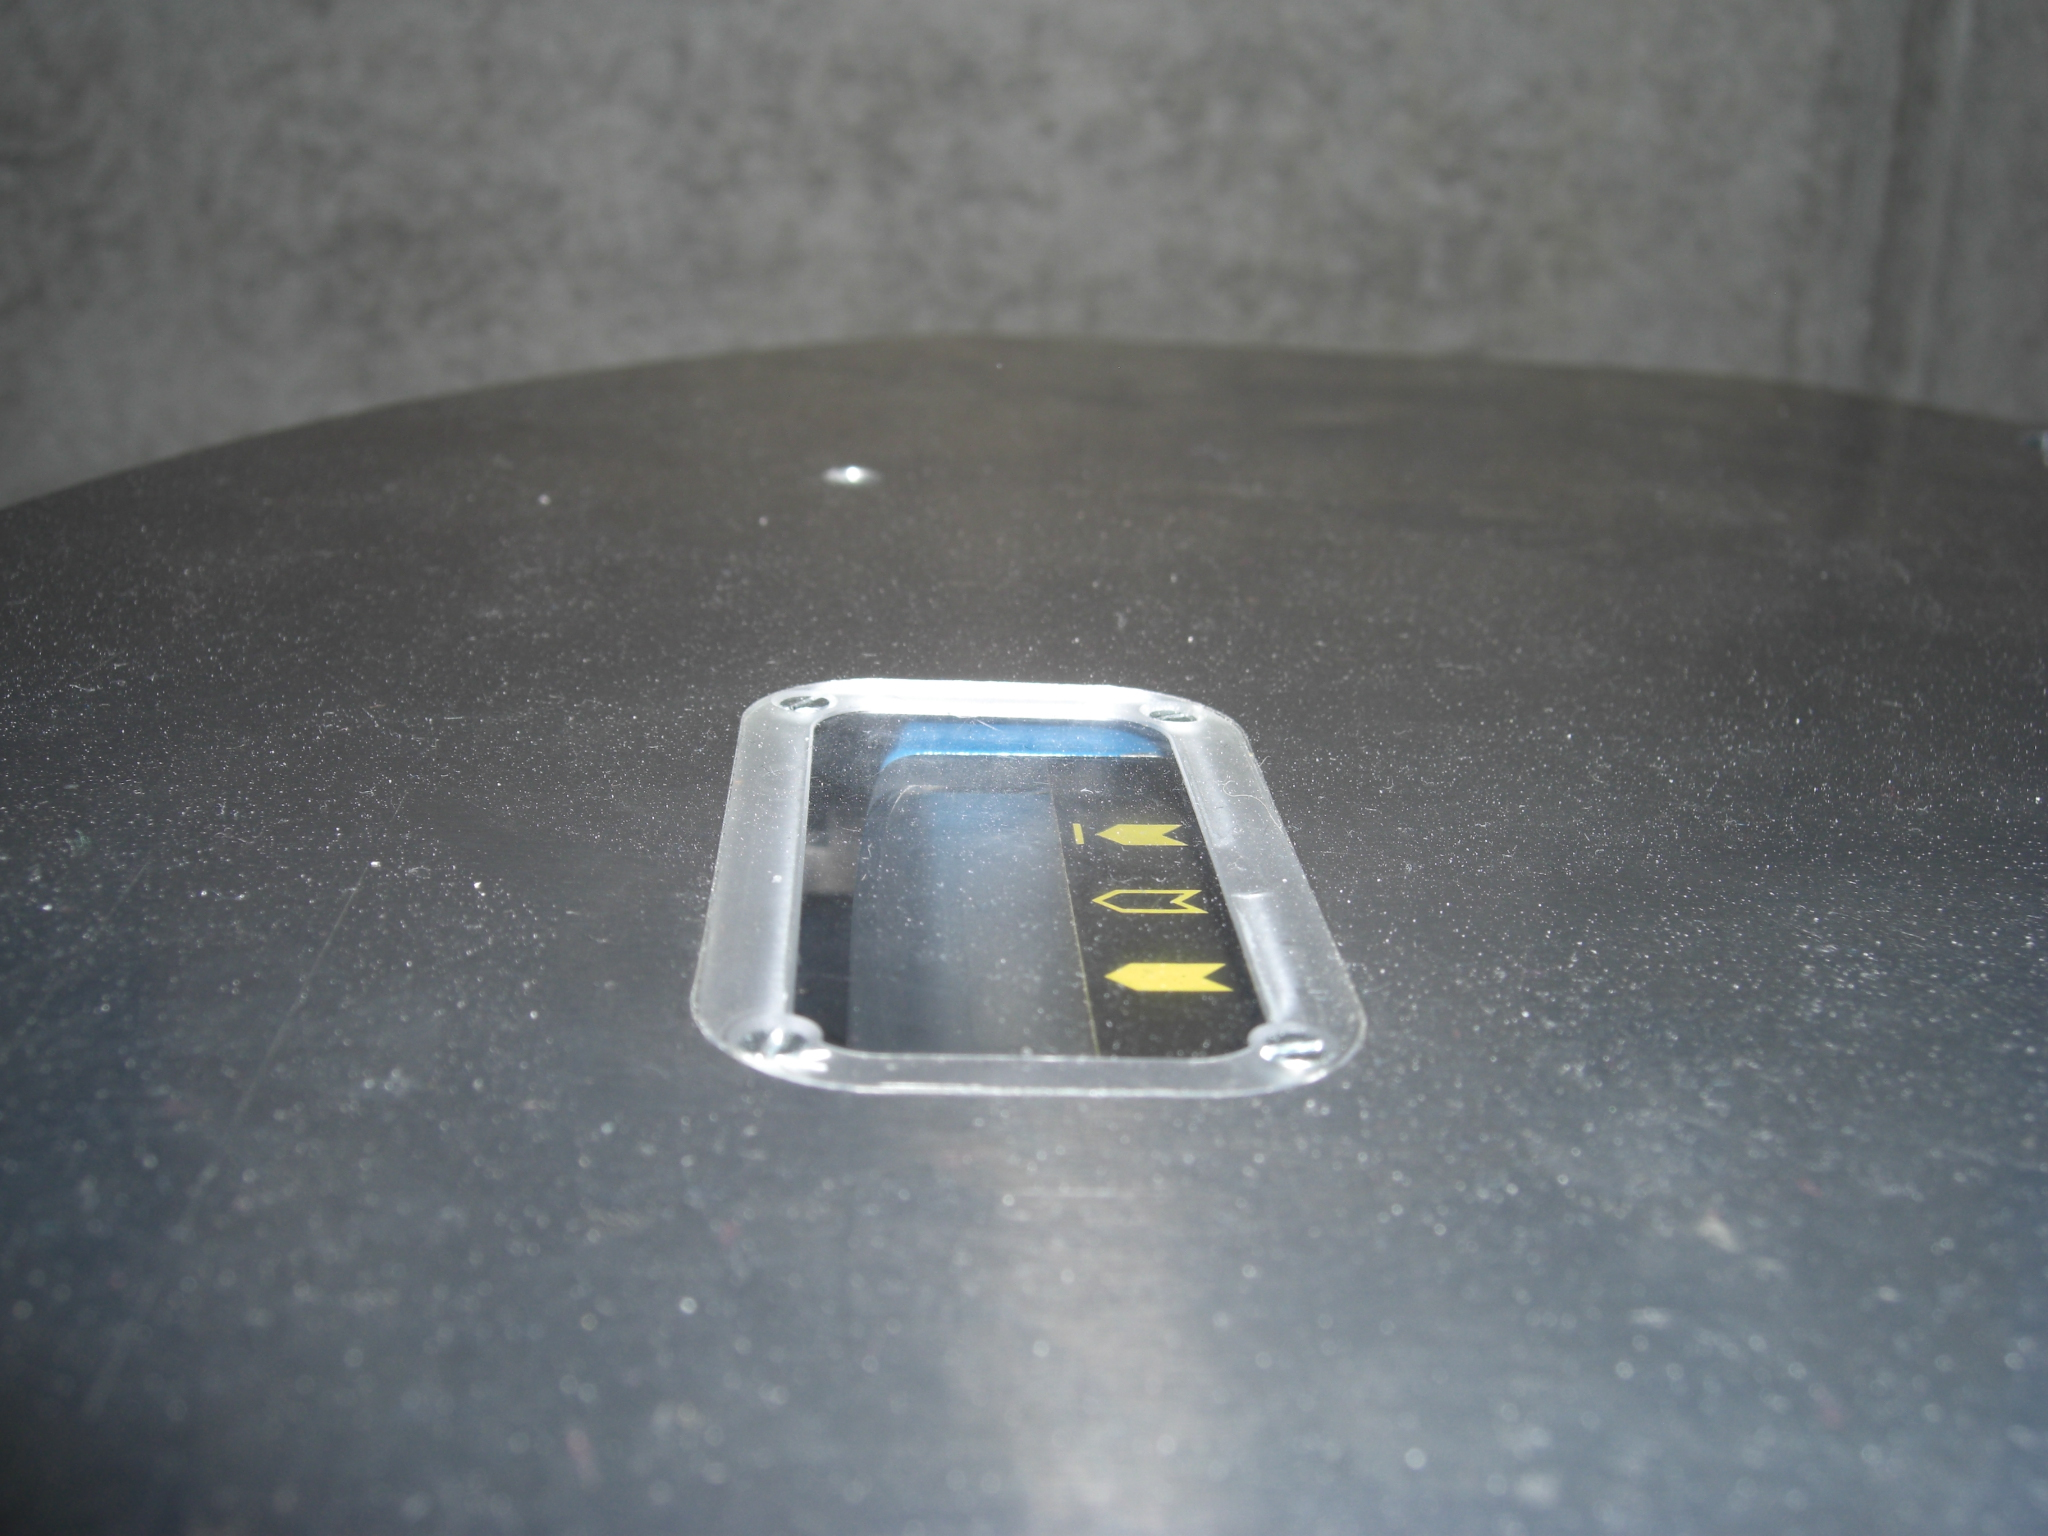
\includegraphics[width=\textwidth/2]{viewing_window.jpg}
  \caption{Viewing Window}
  \label{figure:viewingwindow}
\end{center}
\end{figure}
\begin{figure}[htp]
\begin{center}
  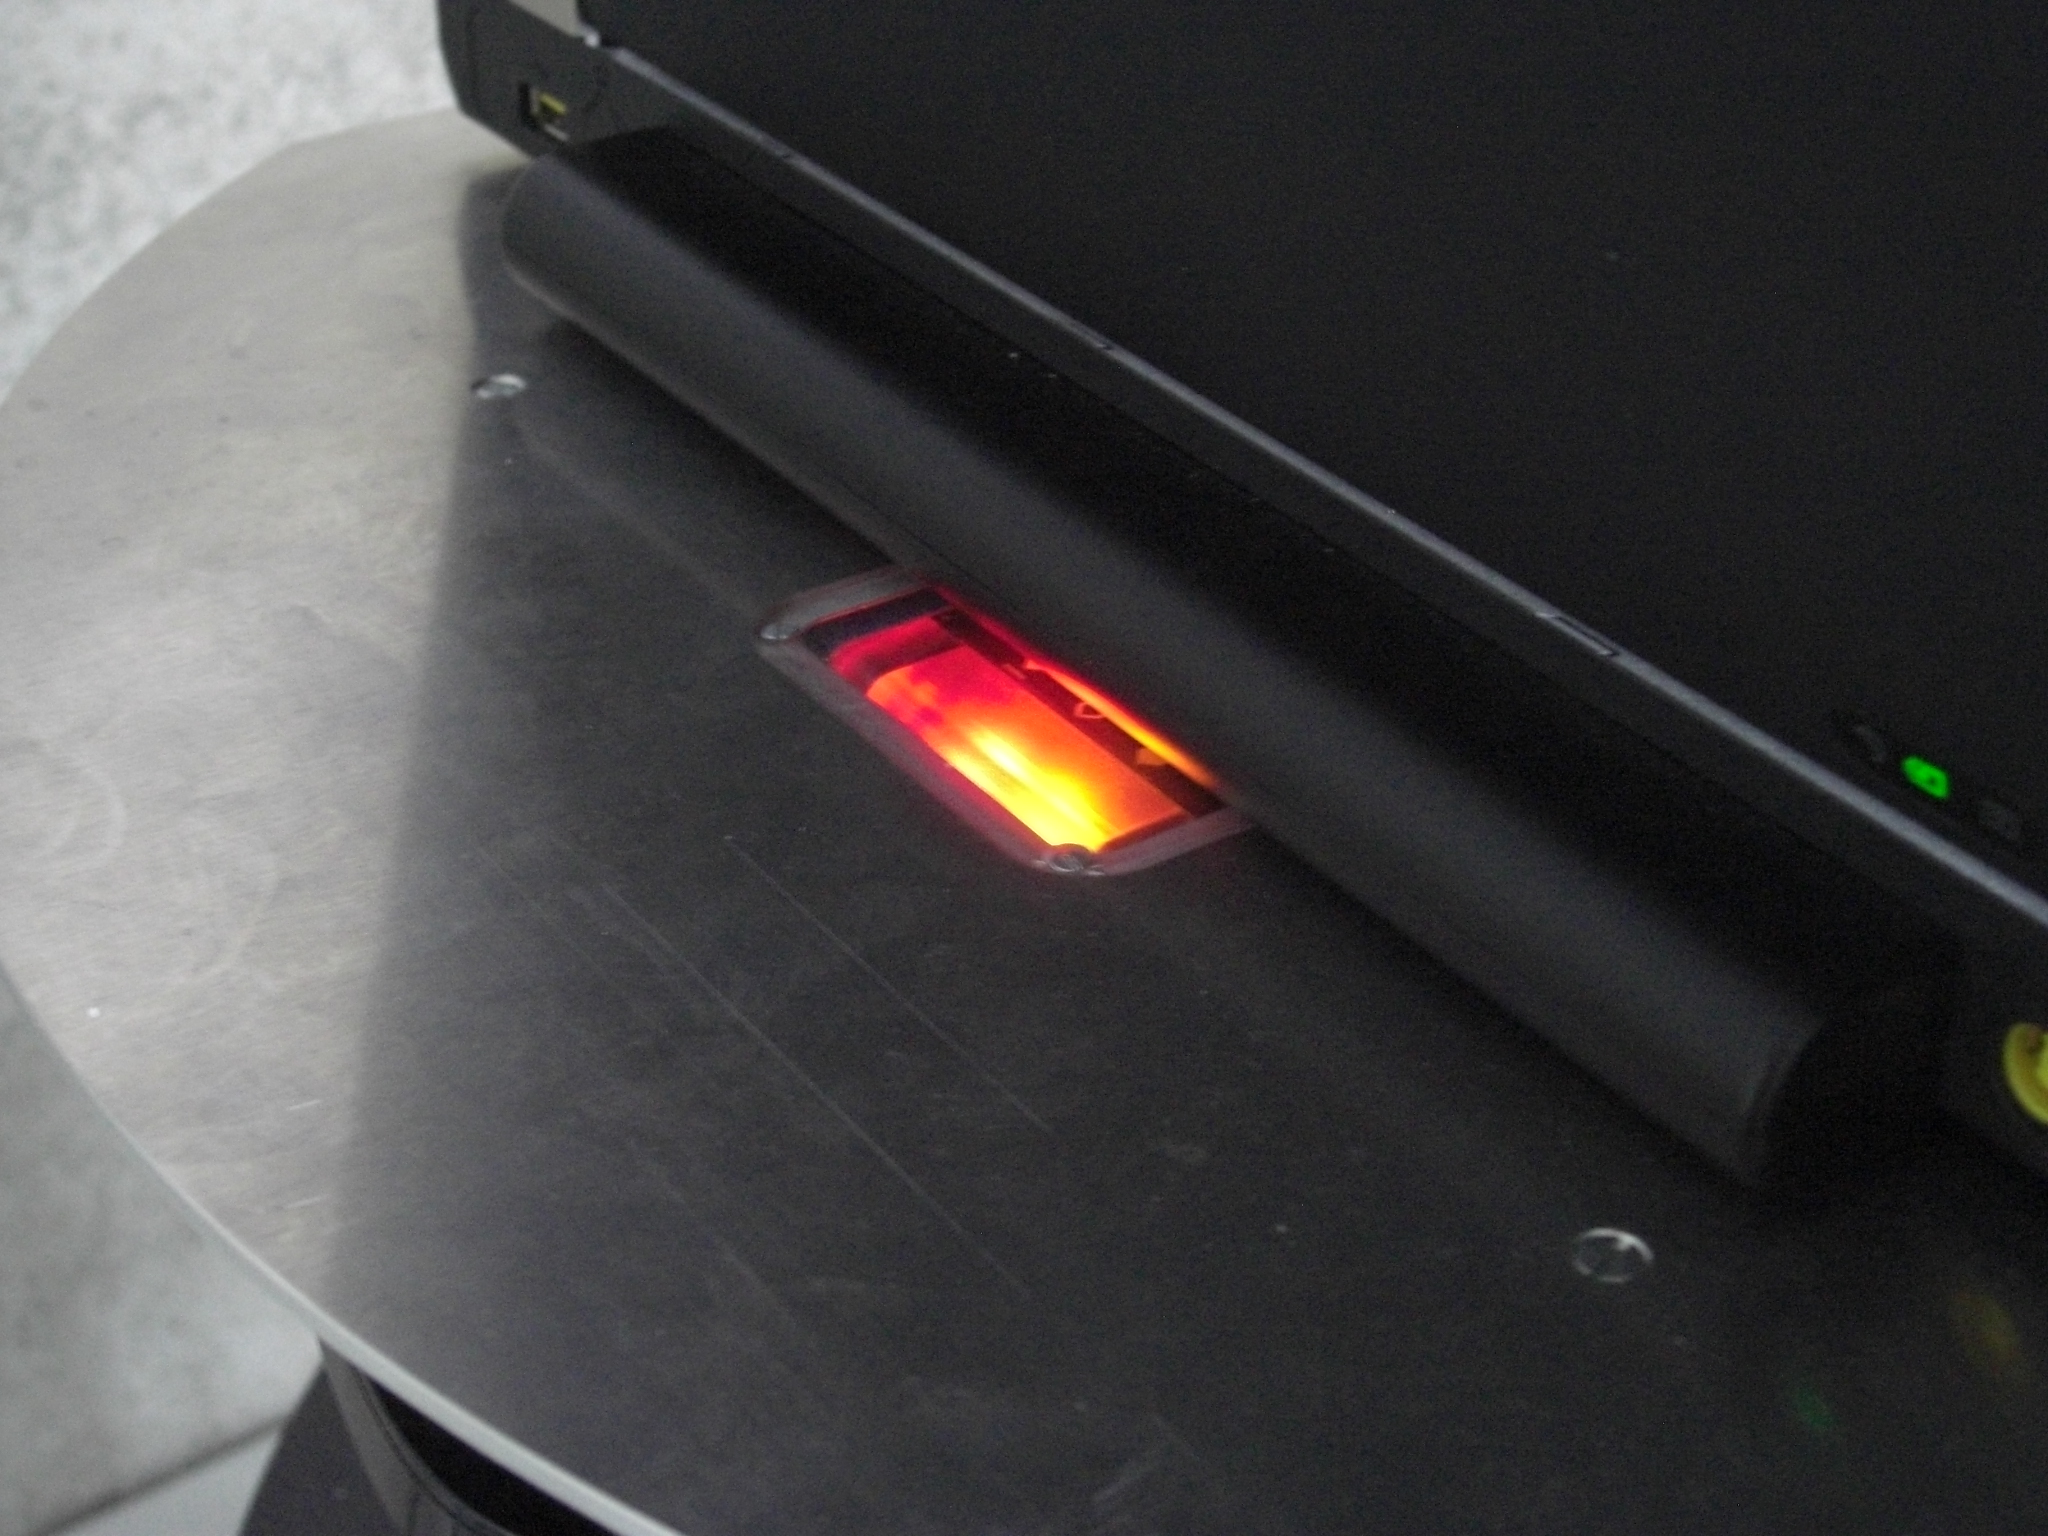
\includegraphics[width=\textwidth/2]{viewing_window_lt.jpg}
  \caption{Viewing Window (with Laptop)}
  \label{figure:viewingwindowlaptop}
\end{center}
\end{figure}
 